\chapter{Conservación de la masa y ecuaciones ajustadas}\label{ch:g8:balanced-equations}

Un tronco de dos kilos \omterm{def:g4:what-a-fire-needs:burning}{arde} en una chimenea. Por la mañana quedan unas
pocas decenas de gramos de ceniza gris. ¿Se esfumaron casi dos kilos de
materia durante la noche? Durante siglos nadie supo responder. La
respuesta llegó de un químico que decidió pesarlo todo, incluidos los
gases que a nadie se le había ocurrido pesar.

\begin{recall}
En una \omterm{def:g7:chemical-reactions:reaction}{reacción química} se consumen los \omterm{def:g7:chemical-reactions:reactant}{reactivos} y se forman los
productos; los \omterm{def:g7:atoms-and-molecules:atom}{átomos} de los \omterm{def:g7:chemical-reactions:reactant}{reactivos} se reorganizan en los productos,
sin crearse ni destruirse (\cref{ch:g7:chemical-reactions}). Una
\omterm{def:g7:atoms-and-molecules:formula}{fórmula química} como \ce{H2O} enumera los \omterm{def:g7:atoms-and-molecules:atom}{átomos} de una \omterm{def:g7:atoms-and-molecules:molecule}{molécula}; un
número delante, como en \ce{3H2O}, cuenta \omterm{def:g7:atoms-and-molecules:molecule}{moléculas}
(\cref{ch:g7:atoms-and-molecules}).
\end{recall}

\begin{omfigure}
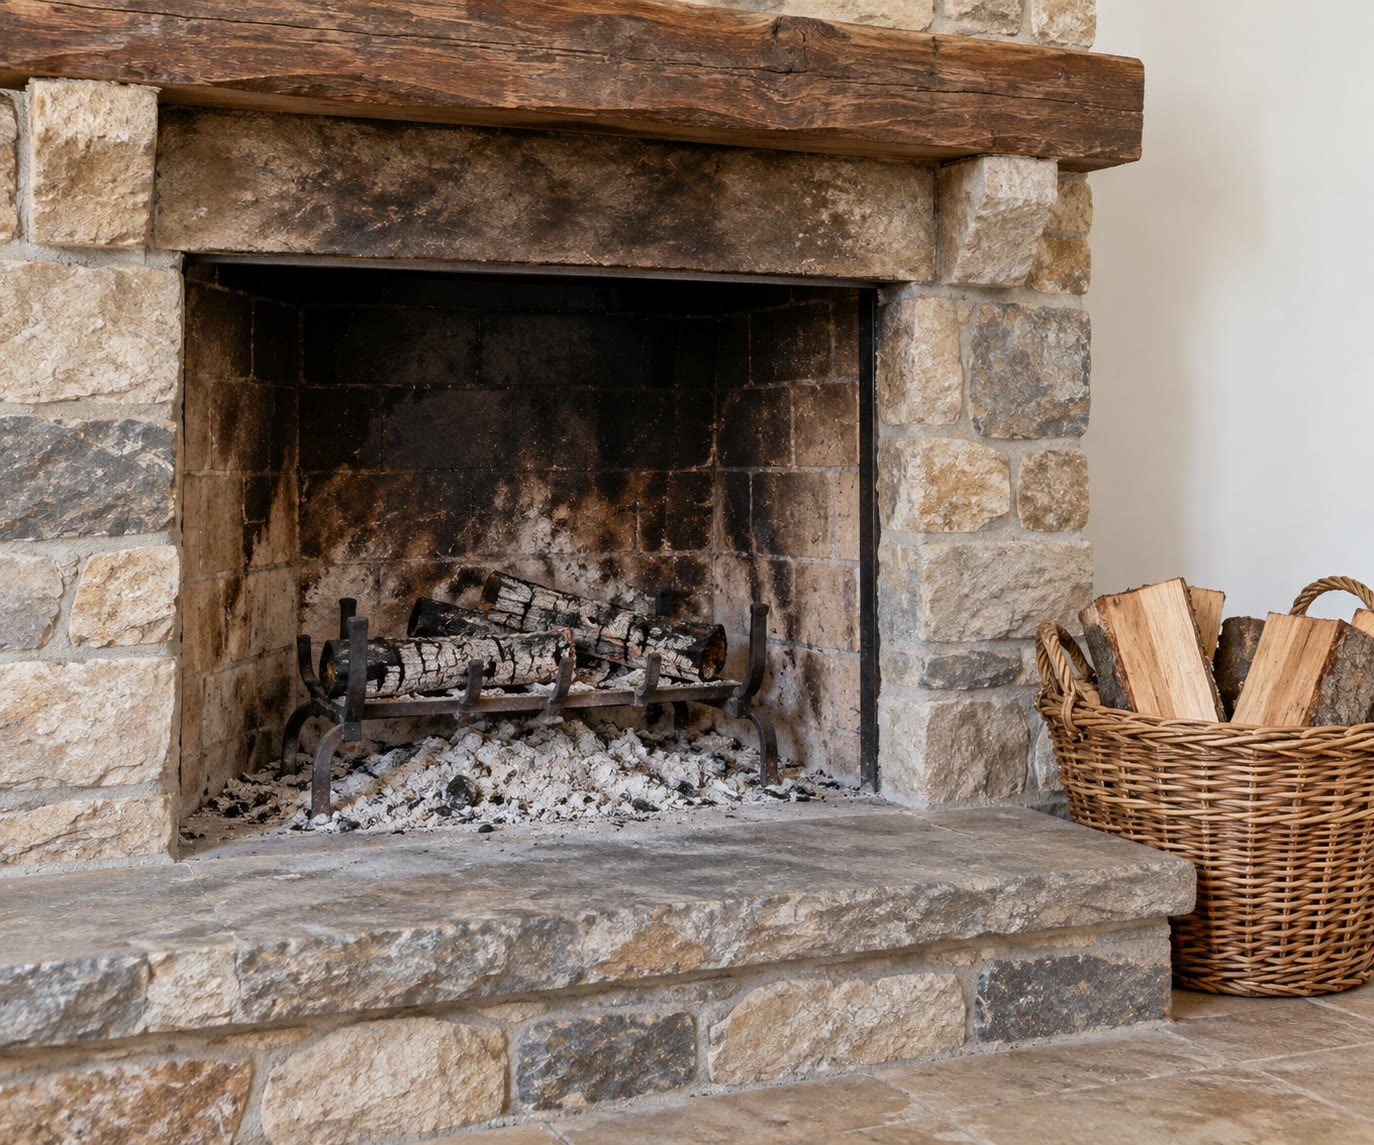
\includegraphics[width=0.5\linewidth]{images/book1/ai/g8-fireplace-ash.jpg}

{\small Una chimenea a la mañana siguiente: de los troncos solo queda un
poco de ceniza.}
\end{omfigure}

\section{La masa se conserva}

\begin{inthelab}[Pesar una reacción en un matraz cerrado]
El profesor pone un poco de vinagre en un matraz, y bicarbonato en un
globo ajustado a su boca, y coloca el conjunto sobre una balanza:
\qty{212.4}{g}. Se levanta el globo para que el bicarbonato caiga en el
vinagre: la \omterm{def:g6:pure-substances-and-mixtures:mixture}{mezcla} burbujea y el globo se hincha con el gas formado. La
balanza sigue marcando \qty{212.4}{g}. La misma reacción en un matraz
abierto, sin el globo, ``pierde'' masa: el gas se escapa a la sala.
\end{inthelab}

\begin{omfigure}
\begin{tikzpicture}[font=\small, scale=1.15]
  % closed flask
  \pic[transform shape] at (0,0) {balance};
  \pic[transform shape] at (0,0.8) {erlenmeyer={0.25}{omWater!80}};
  \fill[red!55, draw=red!60!black] (0,4.05) ellipse (0.5 and 0.62);
  \fill[red!55] (-0.3,3.45) rectangle (0.3,3.6);
  \node[anchor=north, align=center] at (0,-0.1) {cerrado: el gas se queda\\ en el globo};
  \node[anchor=west, font=\footnotesize] at (1.25,0.3) {\qty{212.4}{g}};
  % open flask
  \pic[transform shape] at (4,0) {balance};
  \pic[transform shape] at (4,0.8) {erlenmeyer={0.25}{omWater!80}};
  \foreach \y in {3.6,3.95,4.3} \draw[->, black!45, decorate,
    decoration={snake, amplitude=0.6pt, segment length=4pt}] (4,\y) -- (4,\y+0.3);
  \node[anchor=north, align=center] at (4,-0.1) {abierto: el gas se escapa,\\ la lectura baja};
  \node[anchor=west, font=\footnotesize] at (5.25,0.3) {\qty{211.9}{g}};
\end{tikzpicture}

{\small La misma reacción, pesada. En el matraz cerrado la masa no
cambia; en el matraz abierto el gas se va y la balanza marca menos.}
\end{omfigure}

\begin{definition}[Conservación de la masa]\label{def:g8:balanced-equations:conservation}
La \emph{conservación de la masa}\index{conservacion de la masa@conservación de la masa} es la
ley según la cual, en una \omterm{def:g7:chemical-reactions:reaction}{reacción química}, la masa total de los
productos formados es igual a la masa total de los \omterm{def:g7:chemical-reactions:reactant}{reactivos}
consumidos. No se pierde nada y no se crea nada; la materia solo cambia
de forma.
\end{definition}

\begin{example}[El tronco, bien pesado]\label{ex:g8:balanced-equations:log}
Si se pudieran pesar antes el tronco que \omterm{def:g4:what-a-fire-needs:burning}{arde} y el oxígeno que toma del
\omterm{def:g4:air-a-mixture-of-gases:air}{aire}, y después la ceniza, el dióxido de carbono y el vapor de agua, los
dos totales serían iguales. La ceniza es ligera porque la mayor parte de
los productos son gases que se van por la chimenea.
\end{example}

\begin{history}[Lavoisier lo pesa todo, de 1770 a 1789]
Antoine-Laurent Lavoisier se impuso como norma pesar
todas las sustancias antes y después de cada reacción, en recipientes
cerrados para que ningún gas pudiera salir ni entrar. Demostró que los
metales ganan masa cuando se oxidan o \omterm{def:g4:what-a-fire-needs:burning}{arden}, porque toman algo del \omterm{def:g4:air-a-mixture-of-gases:air}{aire}
(el oxígeno, al que él dio nombre), y afirmó en 1789 que en una
reacción nada se crea y nada se pierde. Su esposa, Marie-Anne Paulze
Lavoisier, trabajaba a su lado, anotaba los experimentos y dibujó los
aparatos para su libro.
\end{history}

\begin{omfigure}
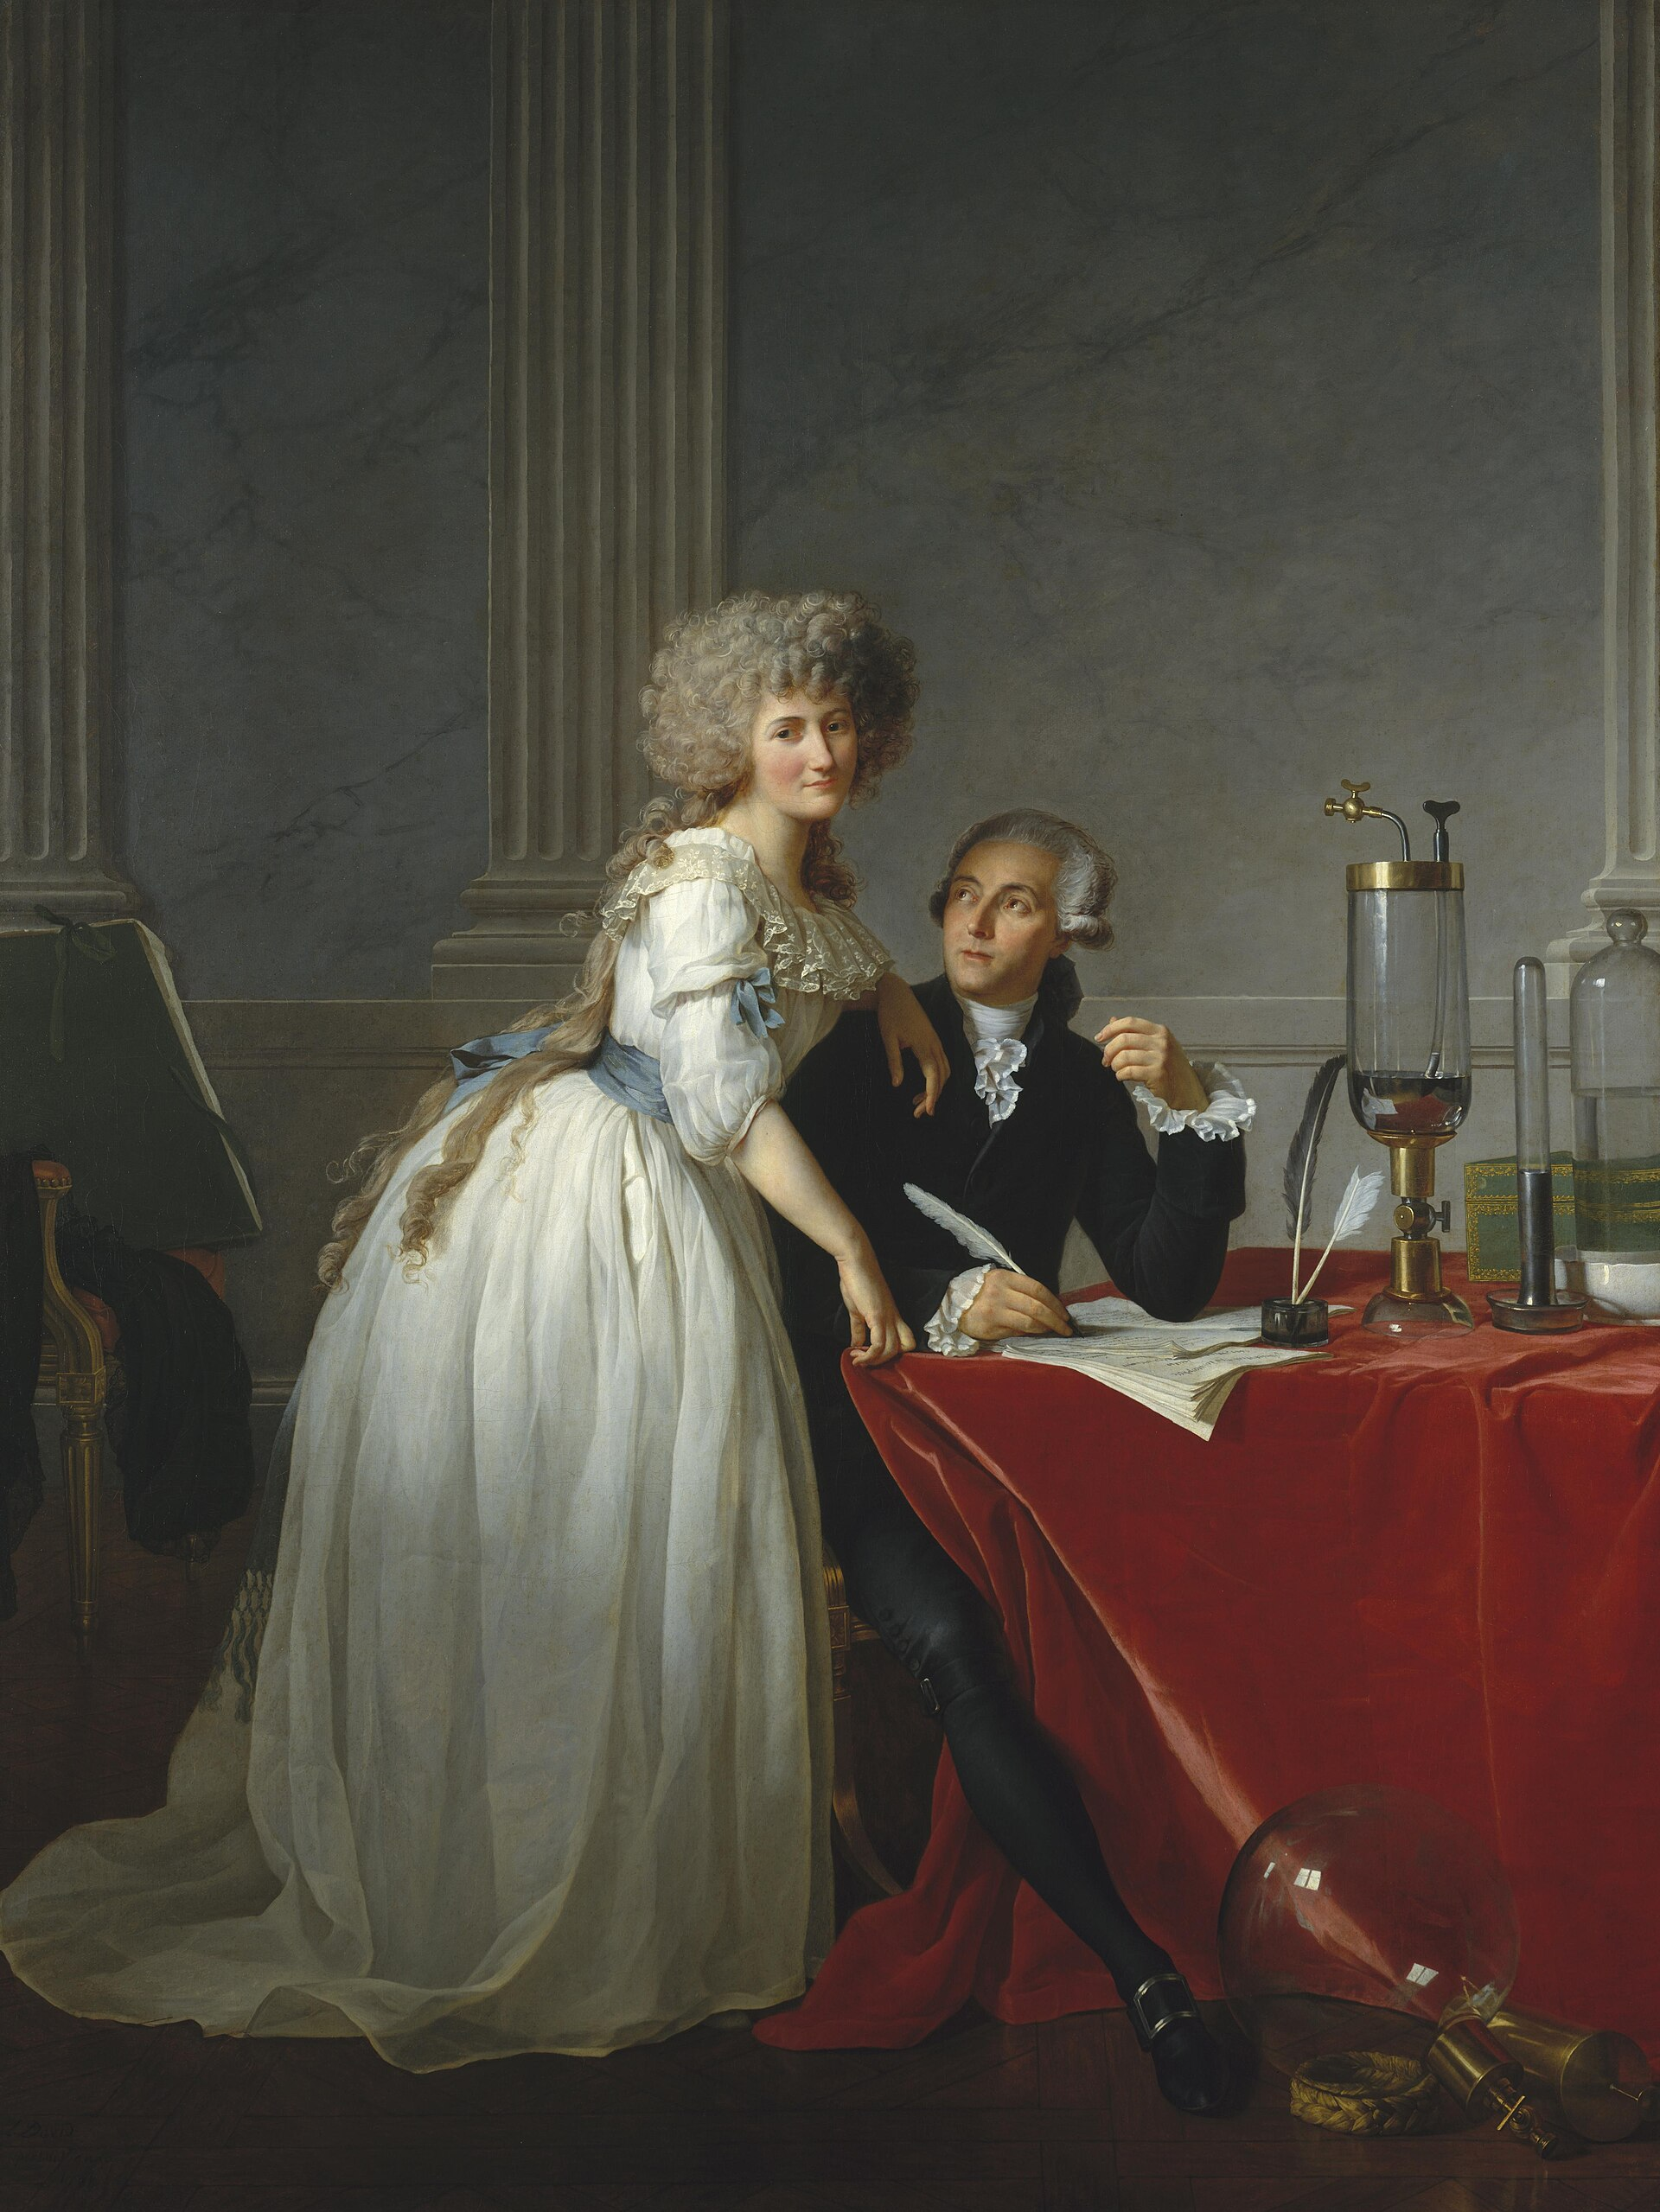
\includegraphics[width=0.3\linewidth]{images/book1/lavoisier.jpg}

{\small Antoine-Laurent Lavoisier y Marie-Anne Paulze Lavoisier, por
Jacques-Louis David, 1788.}
\end{omfigure}

\section{Por qué se conserva la masa}

\begin{proposition}[Los átomos se conservan, así que la masa se conserva]\label{prop:g8:balanced-equations:why}
En una reacción, los \omterm{def:g7:atoms-and-molecules:atom}{átomos} solo se reorganizan: todos los \omterm{def:g7:atoms-and-molecules:atom}{átomos} de
los \omterm{def:g7:chemical-reactions:reactant}{reactivos} se vuelven a encontrar en los productos. Cada \omterm{def:g7:atoms-and-molecules:atom}{átomo}
conserva su propia masa. Por tanto, la masa total no puede cambiar.
\end{proposition}

\begin{example}[Hierro que gana masa]\label{ex:g8:balanced-equations:iron}
La lana de acero quemada sobre una balanza en un recipiente abierto se
vuelve más pesada: los \omterm{def:g7:atoms-and-molecules:atom}{átomos} de hierro se han unido a \omterm{def:g7:atoms-and-molecules:atom}{átomos} de
oxígeno tomados del \omterm{def:g4:air-a-mixture-of-gases:air}{aire}, y el óxido de hierro formado pesa lo que el
hierro más ese oxígeno. Si se quema en un frasco de \omterm{def:g4:air-a-mixture-of-gases:air}{aire} cerrado sobre la
balanza, el conjunto no cambia de masa: el oxígeno ya estaba dentro del
frasco.
\end{example}

\section{La ecuación química}

\begin{definition}[Ecuación química]\label{def:g8:balanced-equations:equation}
Una \emph{ecuación química}\index{ecuacion quimica@ecuación química} escribe una reacción
con fórmulas: las fórmulas de los \omterm{def:g7:chemical-reactions:reactant}{reactivos} a la izquierda, unidas por
$+$, una flecha, y las fórmulas de los productos a la derecha. Cada
fórmula puede llevar un número delante. La ecuación es una
\emph{ecuación ajustada}\index{ecuacion ajustada@ecuación ajustada} cuando cada clase de
\omterm{def:g7:atoms-and-molecules:atom}{átomo} aparece el mismo número de veces en los dos miembros.
\end{definition}

\begin{definition}[Coeficiente estequiométrico]\label{def:g8:balanced-equations:coefficient}
El número escrito delante de una fórmula en una ecuación es su
\emph{coeficiente estequiométrico}\index{coeficiente estequiometrico@coeficiente estequiométrico}:
cuenta las \omterm{def:g7:atoms-and-molecules:molecule}{moléculas} (u otras partículas) de esa especie que
intervienen. El coeficiente 1 no se escribe.
\end{definition}

\begin{notation}[Símbolos de estado]\label{not:g8:balanced-equations:states}
Una letra entre paréntesis después de una fórmula puede indicar su
estado físico: (s) sólido, (l) líquido, (g) gas. Así, \ce{H2O(l)} es el
agua líquida y \ce{H2O(g)}, el vapor de agua.
\end{notation}

\begin{example}[Leer una ecuación]\label{ex:g8:balanced-equations:read}
\[
  \ce{CH4(g) + 2O2(g) -> CO2(g) + 2H2O(l)}
\]
se lee: una \omterm{def:g7:atoms-and-molecules:molecule}{molécula} de metano y dos \omterm{def:g7:atoms-and-molecules:molecule}{moléculas} de oxígeno reaccionan y
dan una \omterm{def:g7:atoms-and-molecules:molecule}{molécula} de dióxido de carbono y dos \omterm{def:g7:atoms-and-molecules:molecule}{moléculas} de agua.
Izquierda: 1 C, 4 H, 4 O. Derecha: 1 C, 4 H, $2 + 2 = 4$ O. La ecuación
está ajustada.
\end{example}

\begin{omfigure}
\begin{tikzpicture}[font=\small]
  \begin{scope}[every node/.style={font=\Large, inner sep=2pt}]
    \node (a) at (0,0) {\ce{CH4}};
    \node (p1) at (0.95,0) {$+$};
    \node (b) at (1.9,0) {\ce{2O2}};
    \node (arr) at (3.35,0) {$\longrightarrow$};
    \node (c) at (4.8,0) {\ce{CO2}};
    \node (p2) at (5.75,0) {$+$};
    \node (d) at (6.8,0) {\ce{2H2O}};
  \end{scope}
  \draw[thick, omDef] ([yshift=-2pt]a.south west) -- ++(0,-0.15) -| ([yshift=-2pt]b.south east);
  \node[below=8pt, text=black] at ($(a.south)!0.5!(b.south)$) {reactivos};
  \draw[thick, omProp] ([yshift=-2pt]c.south west) -- ++(0,-0.15) -| ([yshift=-2pt]d.south east);
  \node[below=8pt, text=black] at ($(c.south)!0.5!(d.south)$) {productos};
  \node[above=6pt of arr, font=\small] {``reaccionan y dan''};
  \node[anchor=north west, align=left, draw=black!35, rounded corners=2pt,
    font=\small, inner sep=4pt] at (-0.3,-1.25)
    {En \ce{2O2}: el 2 grande de delante es el \textbf{coeficiente} (dos moléculas);\\
     el 2 pequeño de abajo es el \textbf{subíndice} (dos átomos en cada molécula).};
\end{tikzpicture}

{\small Las partes de una \omterm{def:g8:balanced-equations:equation}{ecuación química}.}
\end{omfigure}

\section{Ajustar una ecuación}

\begin{method}[Ajustar una ecuación]\label{met:g8:balanced-equations:balance}
\begin{enumerate}
  \item Escribir las fórmulas correctas de los \omterm{def:g7:chemical-reactions:reactant}{reactivos} y de los
        productos. No cambiar nunca una fórmula después: convertir
        \ce{H2O} en \ce{H2O2} describiría otra sustancia.
  \item Contar los \omterm{def:g7:atoms-and-molecules:atom}{átomos} de cada clase en cada miembro.
  \item Ajustar una clase de \omterm{def:g7:atoms-and-molecules:atom}{átomo} cada vez con coeficientes, empezando
        por los \omterm{def:g7:atoms-and-molecules:atom}{átomos} que aparecen en una sola fórmula de cada
        miembro; dejar el hidrógeno y el oxígeno para el final.
  \item Volver a contar; repetir hasta que todas las clases de \omterm{def:g7:atoms-and-molecules:atom}{átomos}
        estén ajustadas.
  \item Usar los números enteros más pequeños.
\end{enumerate}
\end{method}

\begin{example}[Hidrógeno y oxígeno]\label{ex:g8:balanced-equations:water}
Sin ajustar, \ce{H2 + O2 -> H2O} % ce-unbalanced-ok (the skeleton)
tiene 2 O a la izquierda y 1 a la derecha. Ponemos un 2 delante de
\ce{H2O}: ahora hay 4 H a la derecha, así que ponemos un 2 delante de
\ce{H2}:
\[
  \ce{2H2 + O2 -> 2H2O}.
\]
Comprobación: 4 H y 2 O en cada miembro.
\end{example}

\begin{example}[El hierro arde en oxígeno]\label{ex:g8:balanced-equations:iron-oxide}
El hierro y el oxígeno dan el óxido de hierro \ce{Fe2O3}. Oxígeno: 2 a
la izquierda, 3 a la derecha; el menor número común es 6, así que 3
\ce{O2} y 2 \ce{Fe2O3}. Entonces hay 4 Fe a la derecha, así que 4 Fe a
la izquierda:
\[
  \ce{4Fe + 3O2 -> 2Fe2O3}.
\]
\end{example}

\begin{omfigure}
\begin{tikzpicture}[font=\small]
  % 2 H2
  \foreach \y in {0.45,-0.45} {
    \node[aH] (a) at (0,\y) {}; \node[aH] (b) at (0.45,\y) {};
    \begin{scope}[on background layer]\draw[bond] (a.center) -- (b.center);\end{scope}}
  \node at (1.05,0) {$+$};
  \node[aO] (a) at (1.6,0) {}; \node[aO] (b) at (2.25,0) {};
  \begin{scope}[on background layer]
    \draw[bond, line width=1.1pt] ([yshift=1.6pt]a.center) -- ([yshift=1.6pt]b.center);
    \draw[bond, line width=1.1pt] ([yshift=-1.6pt]a.center) -- ([yshift=-1.6pt]b.center);
  \end{scope}
  \draw[->, thick, omProp] (2.9,0) -- (3.9,0);
  \foreach \y in {0.5,-0.5} {
    \node[aO] (o) at (4.9,\y+0.12) {};
    \node[aH] (p) at (4.35,\y-0.28) {}; \node[aH] (q) at (5.45,\y-0.28) {};
    \begin{scope}[on background layer]
      \draw[bond] (o.center) -- (p.center); \draw[bond] (o.center) -- (q.center);
    \end{scope}}
  \node[align=center, font=\footnotesize] at (1.1,-1.35) {4 H, 2 O};
  \node[align=center, font=\footnotesize] at (4.9,-1.35) {4 H, 2 O};
  \node[font=\small] at (2.7,-2.0) {\ce{2H2 + O2 -> 2H2O}};
\end{tikzpicture}

{\small La \omterm{def:g8:balanced-equations:equation}{ecuación ajustada} de la \omterm{def:g4:what-a-fire-needs:burning}{combustión} del hidrógeno, dibujada
con modelos: dos \omterm{def:g7:atoms-and-molecules:molecule}{moléculas} de hidrógeno y una \omterm{def:g7:atoms-and-molecules:molecule}{molécula} de oxígeno dan
dos \omterm{def:g7:atoms-and-molecules:molecule}{moléculas} de agua.}
\end{omfigure}

\section{Leer una ecuación en moléculas}


\begin{proposition}[Lo que dice una ecuación ajustada]\label{prop:g8:balanced-equations:molecules}
Los coeficientes de una \omterm{def:g8:balanced-equations:equation}{ecuación ajustada} dan las proporciones en que
reaccionan y se forman las partículas. Si la ecuación es
\ce{2H2 + O2 -> 2H2O}, 200 \omterm{def:g7:atoms-and-molecules:molecule}{moléculas} de hidrógeno reaccionan con 100
\omterm{def:g7:atoms-and-molecules:molecule}{moléculas} de oxígeno y dan 200 \omterm{def:g7:atoms-and-molecules:molecule}{moléculas} de agua; un millón de \omterm{def:g7:atoms-and-molecules:molecule}{moléculas}
de oxígeno necesitan dos millones de \omterm{def:g7:atoms-and-molecules:molecule}{moléculas} de hidrógeno.
\end{proposition}

\begin{example}[El propano de un hornillo de camping]\label{ex:g8:balanced-equations:propane}
El propano, \ce{C3H8}, \omterm{def:g4:what-a-fire-needs:burning}{arde} en oxígeno y da dióxido de carbono y agua.
Primero el carbono: 3 C, así que 3 \ce{CO2}. El hidrógeno: 8 H, así que
4 \ce{H2O}. El oxígeno de la derecha: $3 \times 2 + 4 = 10$ O, así que
5 \ce{O2}:
\[
  \ce{C3H8 + 5O2 -> 3CO2 + 4H2O}.
\]
Cada \omterm{def:g7:atoms-and-molecules:molecule}{molécula} de propano necesita cinco \omterm{def:g7:atoms-and-molecules:molecule}{moléculas} de oxígeno.
\end{example}

\section{Ejercicios}

\begin{exercise}[$\star$]\label{exo:g8:balanced-equations:1}
Enuncia la ley de \omterm{def:g8:balanced-equations:conservation}{conservación de la masa}.
\end{exercise}

\begin{exercise}[$\star$]\label{exo:g8:balanced-equations:2}
En \ce{3CO2}, ¿cuál es el \omterm{def:g8:balanced-equations:coefficient}{coeficiente estequiométrico}? ¿Cuántos \omterm{def:g7:atoms-and-molecules:atom}{átomos}
de carbono y cuántos \omterm{def:g7:atoms-and-molecules:atom}{átomos} de oxígeno representa?
\end{exercise}

\begin{exercise}[$\star$]\label{exo:g8:balanced-equations:3}
¿Está ajustada \ce{C + O2 -> CO2}? Cuenta los \omterm{def:g7:atoms-and-molecules:atom}{átomos} para comprobarlo.
\end{exercise}

\begin{exercise}[$\star$]\label{exo:g8:balanced-equations:4}
Ajusta \ce{Mg + O2 -> MgO}. % ce-unbalanced-ok (to balance)
\end{exercise}

\begin{exercise}[$\star\star$]\label{exo:g8:balanced-equations:5}
Ajusta \ce{N2 + H2 -> NH3}, la reacción con la que se fabrica el amoniaco. % ce-unbalanced-ok (to balance)
\end{exercise}

\begin{exercise}[$\star\star$]\label{exo:g8:balanced-equations:6}
\qty{12}{g} de carbono \omterm{def:g4:what-a-fire-needs:burning}{arden} por completo y forman \qty{44}{g} de
dióxido de carbono. ¿Qué masa de oxígeno se ha consumido?
\end{exercise}

\begin{exercise}[$\star\star$]\label{exo:g8:balanced-equations:7}
Mira la figura de los dos matraces sobre balanzas. ¿Por qué baja la
lectura del matraz abierto? ¿Se ha destruido masa?
\end{exercise}

\begin{exercise}[$\star\star$]\label{exo:g8:balanced-equations:8}
Ajusta \ce{CH4 + O2 -> CO2 + H2O} paso a paso, diciendo qué \omterm{def:g7:atoms-and-molecules:atom}{átomo} % ce-unbalanced-ok (to balance)
ajustas en cada paso.
\end{exercise}

\begin{exercise}[$\star\star$]\label{exo:g8:balanced-equations:9}
Un alumno ajusta \ce{H2 + O2 -> H2O} escribiendo \ce{H2 + O2 -> H2O2}. % ce-unbalanced-ok (the student's start)
¿Por qué está mal?
\end{exercise}

\begin{exercise}[$\star\star$]\label{exo:g8:balanced-equations:10}
Con \ce{C3H8 + 5O2 -> 3CO2 + 4H2O}, ¿cuántas \omterm{def:g7:atoms-and-molecules:molecule}{moléculas} de oxígeno hacen
falta para quemar 20 \omterm{def:g7:atoms-and-molecules:molecule}{moléculas} de propano? ¿Cuántas \omterm{def:g7:atoms-and-molecules:molecule}{moléculas} de agua se
forman?
\end{exercise}

\begin{exercise}[$\star\star\star$]\label{exo:g8:balanced-equations:11}
Ajusta \ce{C2H6 + O2 -> CO2 + H2O}, la \omterm{def:g4:what-a-fire-needs:burning}{combustión} del etano. (Pista: % ce-unbalanced-ok (to balance)
prueba a duplicar el etano.)
\end{exercise}

\begin{exercise}[$\star\star\star$]\label{exo:g8:balanced-equations:12}
Una vela de \qty{20.0}{g} \omterm{def:g4:what-a-fire-needs:burning}{arde} dentro de una caja de vidrio cerrada
llena de \omterm{def:g4:air-a-mixture-of-gases:air}{aire}, colocada sobre una balanza que marca \qty{850.0}{g} en
total. Cuando la llama se apaga, la vela pesa \qty{19.6}{g}. ¿Qué marca
la balanza? Explícalo.
\end{exercise}

\section{Problema: Lana de acero en un frasco cerrado}

\begin{problem}[{Problema de fin de semana --- un hierro que arde, una
balanza que no se mueve y el oxígeno tomado del aire}]
\label{pb:g8:balanced-equations:1}
En un laboratorio, un profesor quema lana de acero, que es hierro casi
puro, de dos maneras. Primero quema un estropajo en un recipiente
abierto sobre una balanza: la lectura sube. Después quema un estropajo
de \qty{0.28}{g}, encendido con una chispa eléctrica, dentro de un
frasco cerrado lleno de \omterm{def:g4:air-a-mixture-of-gases:air}{aire} colocado sobre la balanza: la lectura no
cambia. El frasco contiene alrededor de \qty{0.5}{g} de oxígeno. El
hierro que \omterm{def:g4:what-a-fire-needs:burning}{arde} en oxígeno forma el óxido de hierro \ce{Fe2O3}; con
menos oxígeno también puede formar \ce{Fe3O4}.

\medskip
\noindent\textbf{Parte I --- Dos pesadas.}
\begin{enumerate}
  \item En el recipiente abierto, la masa aumenta. ¿De dónde viene la
        masa adicional?
  \item En el frasco cerrado, la masa no cambia. Explícalo.
  \item Enuncia la ley que ilustran estas dos pesadas.
\end{enumerate}

\medskip
\noindent\textbf{Parte II --- Dos ecuaciones.}
\begin{enumerate}[resume]
  \item Ajusta la ecuación \ce{Fe + O2 -> Fe2O3}. % ce-unbalanced-ok (to balance)
  \item Ajusta la ecuación \ce{Fe + O2 -> Fe3O4}. % ce-unbalanced-ok (to balance)
  \item Comprueba la primera ecuación contando los \omterm{def:g7:atoms-and-molecules:atom}{átomos} de cada clase
        en cada miembro.
  \item Según la primera ecuación, ¿cuántas \omterm{def:g7:atoms-and-molecules:molecule}{moléculas} de oxígeno
        reaccionan con 400 \omterm{def:g7:atoms-and-molecules:atom}{átomos} de hierro?
\end{enumerate}

\medskip
\noindent\textbf{Parte III --- Masas.}
En el \ce{Fe2O3}, cada \qty{7}{g} de hierro están combinados con
\qty{3}{g} de oxígeno. El estropajo de \qty{0.28}{g} \omterm{def:g4:what-a-fire-needs:burning}{arde} por completo y
se convierte en \ce{Fe2O3}.
\begin{enumerate}[resume]
  \item ¿Qué masa de oxígeno se combina con \qty{0.28}{g} de hierro?
  \item ¿Cuál es la masa de óxido de hierro formada?
  \item ¿Había suficiente oxígeno en el frasco? Explícalo.
  \item Se abre el frasco después de que se enfríe, y entra \omterm{def:g4:air-a-mixture-of-gases:air}{aire} de
        golpe. Explica por qué, y di cómo cambia entonces la lectura de
        la balanza.
  \item Calcula la masa de oxígeno que la lana de acero, al \omterm{def:g4:what-a-fire-needs:burning}{arder}, ha
        tomado del \omterm{def:g4:air-a-mixture-of-gases:air}{aire} del frasco.
\end{enumerate}
\end{problem}
